\documentclass[a4paper]{article}

\usepackage[english]{babel}
\usepackage[utf8]{inputenc}
\usepackage{fullpage}
\usepackage{amsmath}
\usepackage{graphicx}
\usepackage[colorinlistoftodos]{todonotes}
%\usepackage{hyperref}
\usepackage{amssymb}
\usepackage{subfigure}
\usepackage{url}
\usepackage[pagebackref=true,colorlinks,linkcolor=red,citecolor=green,breaklinks=true,bookmarks=false]{hyperref}
\usepackage{outline} 
\usepackage{pmgraph} \usepackage[normalem]{ulem}
\usepackage{graphicx} \usepackage{verbatim}
\usepackage{indentfirst}
\usepackage{listings}
\usepackage{xcolor}
\setlength{\parindent}{2em}
% \usepackage{minted} % need `-shell-escape' argument for local compile

\title{
    \vspace*{1in}
    
\includegraphics[width=2.75in]{figures/zhenglab-logo} \\
    \vspace*{1.2in}
    \textbf{\huge Weekly Work Report}
    \vspace{0.2in}
}

\author{Hongzhi Liu \\
    \vspace*{0.5in} \\
    \textbf{VISION@OUC} \\
    \vspace*{1in}
}

\date{\today}


\begin{document}
\par
\maketitle
\setcounter{page}{0}
\thispagestyle{empty}

\newpage

\section{Research problem}

During this period of week, I spend time studying deep learning courses and working about Faster R-CNN algorithm and flow guided feature aggregation for video object detection method in order to prepare URPC2018. Our team try to let code program output relevant documents to evaluate algorithm performance. Besides, I receive three kinds of image restoration datasets to train a model and test how good the restoration algorithm are.

Because of code modification, I have difficulty in adding codes to realize the function which can output a txt which includes information about picture ID, class, confidence and bounding box. Besides, I need to rectify and debug the relevant codes of algorithm until they can meet the requirement to test and evaluate a contest model. At last, I should build a simulation environment for flow guided feature aggregation. 

\section{Research approach}

In the process of research, I use the method of documentary analysis, comparative analysis and experimental research method. I read the thesis of Fast R-CNN \cite{Girshick2015Fast}, Faster R-CNN algorithm \cite{Ren2015Faster} and flow guided feature aggregation \cite{zhu17fgfa}. I try to unferstand core ideology in paper and learn about concept introduced by author.

Besides, I need to clone codes from github which shared by other researcher. Then I debug and run the demo program to learn how to realize an algorithm which can be called experimental method. 

For deep learning, I watch videos and write down the issues which I think are much important for further research. And then, I not only have learned the lessons of deep learning, but also put them into code editing action. 


\section{Research progress}

During preparation for URPC2018, I receive three kinds of image restoration datasets to train a model and test how good the restoration algorithm are. I continue to learn about Faster R-CNN algorithm \cite{Ren2015Faster} and  relevant codes of flow guided feature aggregation \cite{zhu17fgfa}. Furthermore, I receive three datasets which have been image restored. By using the remote server, I try to train three knids of contest models with data sets and test how well model run. I will list details about weekly work in Tab.~\ref{t1} below. 

\begin{table}[hb]
	\centering
	\caption{Weekly work progress.}
	\begin{tabular}{c|p{10cm}}
		\hline 
		& Finish reading paper flow-guided feature aggregation for video object detection written by Xizhou Zhu \emph{et al.}.\\
		
		URPC2018 & Finish changing size of restored image from 256$\times$ 256 to original size. \\
		
		& Finish training three kinds of models with image restoration data sets.\\
		
		& Succeed in outputting the txt to meet the requirement of contest.\\
		\hline
		& Finish learning improving deep neural network course: Hyperparameter tuning, regularization and optimization, which is the second lesson \\
		Deep learning courses & Finish learning structuring machine learning projects which is the third lesson. \\
		\hline
	\end{tabular}
	\label{t1}
\end{table} 


\section{Progress in this week}

During preparation for URPC2018, I have learned to do some relevant work in order to achieve the goal of contest. Our team adopt three different kinds of image restoration methods to produce three data sets which have been used to train models. And I have succeed in outputting the txt to meet the requirement of contest. The progress has been maked at the present stage as shown in table blow.
\begin{description}
	\item [Step 1] Finish changing size of restored images from 256$\times$ 256 to original size.
	\item[Step 2] Finish training three kinds of models with image restoration data sets.
	\item[Step 3] Finish outputting the txt to meet the requirement of contest.
	\item[Step 4] structuring machine learning projects which is the third lesson.\label{t2}
\end{description}

\subsection{Data Sets}
In this week, my colleague in our team adopt three different kinds of image restoration methods to produce three data sets, which can be called cla2, cla6 and hsv just as shown in Fig.~\ref{p1}. Then I change thousands of pictures into VOC2007 format which is necessary for training. Fig.~\ref{p1}\subref{p1a} is the picture restored by cla2 method, Fig.~\ref{p1}\subref{p1b} is the picture restored by cla6 method and Fig.~\ref{p1}\subref{p1c} is the picture restored by hsv method.

Because the image sizes of restored picture is different from xml files which have been made last week, I need to change size of restored images from 256$\times$ 256 to original size by coding script files in \ref{g1}.
\begin{figure}[!b]
	\centering 
	\subfigure[]{ 
		\label{p1a} %% label for first subfigure 
		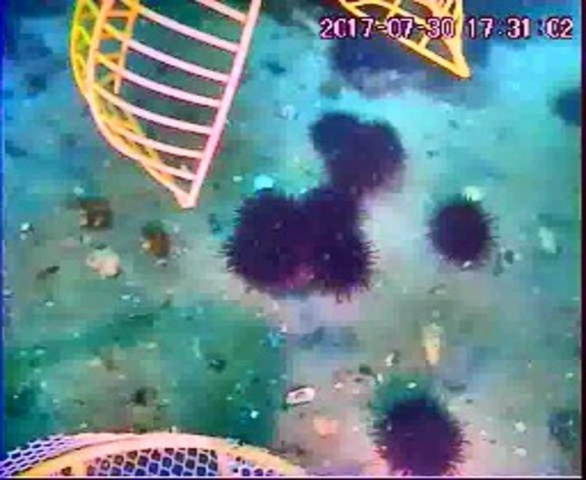
\includegraphics[width=4cm]{figures/1.jpg} 
	} 
	\subfigure[]{ 
		\label{p1b} %% label for second subfigure 
		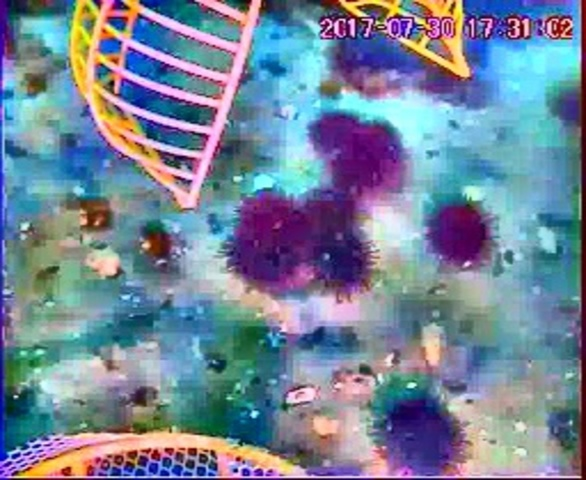
\includegraphics[width=4cm]{figures/2.jpg} 
	} 
	\subfigure[]{ 
		\label{p1c} %% label for second subfigure 
		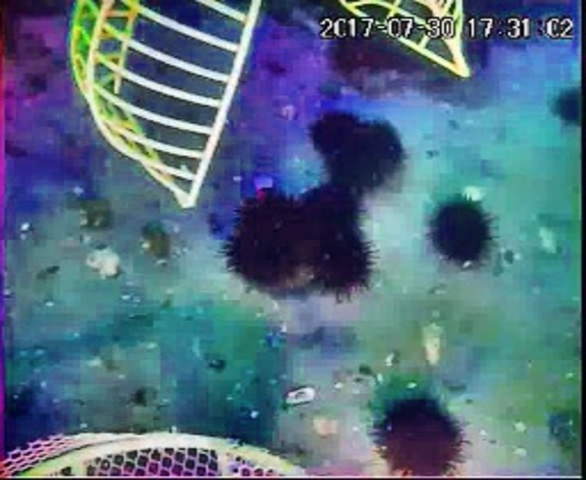
\includegraphics[width=4cm]{figures/3.jpg} 
	} 
	\caption{Three kinds of image restoration.} 
	\label{p1} %% label for entire figure 
\end{figure}

\lstset{language=bash}
\begin{lstlisting}
set -e  # or use "set -o errexit" to quit on error.
set -x  # or use "set -o xtrace" to print the statement before you execute it.

FILES=*.jpg
for f in $FILES
do
echo "$f"
convert $f -resize 586x480! $f
done  
\end{lstlisting}\label{g1}

\subsection{Train a Contest Model}

We put restored picture data sets to the remote server and try to train a model that can meet requirement of contest. Before doing like this, appropriate code modification is necessary because self.classes and label is not as same as VOC. In the project of Faster R-CNN files, relevant codes in pascal\_voc.py need to revise, for example contents in self.\_classes variable has become what we want that are holothurian, echinus, scallop and starfish.

I train the contest model from Tuesday to Friday on the server. Then I run demo.py to test the performance of model as shown in Fig.~\ref{p2}. Fig.~\ref{p2}\subref{p2a} is experimental results of cla2, Fig.~\ref{p2}\subref{p2b} is experimental results of cla6, and Fig.~\ref{p2}\subref{p2c} is experimental results of hsv.
\begin{figure}
	\centering 
	\subfigure[]{ 
		\label{p2a} %% label for first subfigure 
		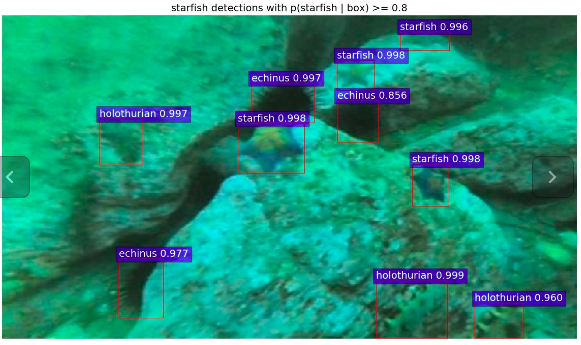
\includegraphics[width=5cm]{figures/4.png} 
	} 
	\subfigure[]{ 
		\label{p2b} %% label for second subfigure 
		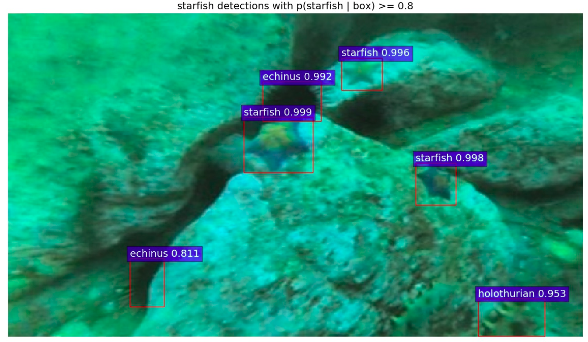
\includegraphics[width=5cm]{figures/5.png} 
	}
	\subfigure[]{ 
		\label{p2c} %% label for second subfigure 
		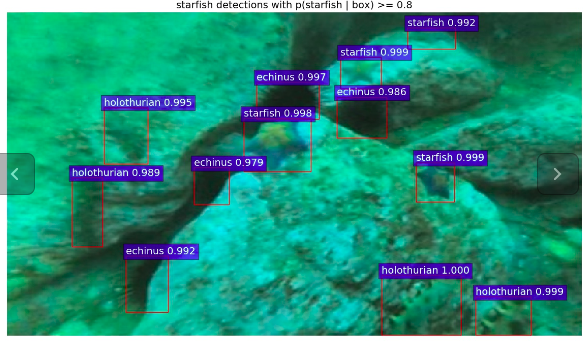
\includegraphics[width=5cm]{figures/6.png} 
	} 
	\caption{Experimental results of the contest model.} 
	\label{p2} %% label for entire figure 
\end{figure}

\begin{figure}[!b]
	\begin{center}
		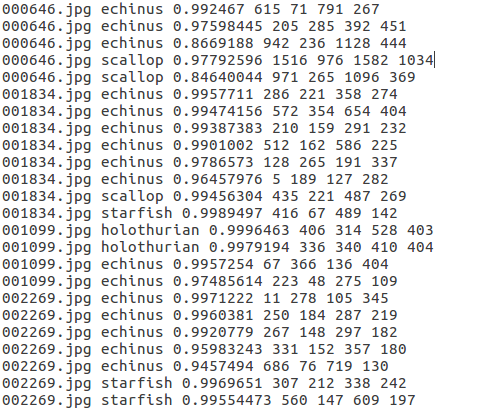
\includegraphics[scale=0.4]{figures/7.png}
	\end{center}
	\caption{Output file in contest format.}
	\label{p3}
\end{figure}

Furthermore, I should check total loss of my model to learn more about my model. Simulation results prove that this improved algorithm achieves an effect in accelerating the converging rate.

\subsection{Outputs of Contest Format}

From the instruction of contest, we need to submit a test which conbines $<image\_id> <class\_id> <confidence> <xmin> <ymin> <xmax> <ymax>$. So I learn to write txt and succeed in outputting the standard file and the codes which I add is in following part \ref{g2}. Besides, the output file can be seen in Fig.~\ref{p3}.
\lstset{language=python}
\begin{lstlisting}
   for i in inds:
   bbox = dets[i, :4]
   score = dets[i, -1]
   if class_name == '__background__':
   fw = open('result.txt', 'a')  
   fw.write(str(im_name) + ' ' + class_name + ' ' + str(score) + ' ' +str(int(bbox[0])) + ' ' + str(int(bbox[1])) + ' ' + str(int(bbox[2])) + ' ' + str(int(bbox[3])) + '\n')
   fw.close()
   
   elif class_name == 'holothurian':
   fw = open('result.txt', 'a')  
   fw.write(str(im_name) + ' ' + class_name + ' ' + str(score) + ' ' +str(int(bbox[0])) + ' ' + str(int(bbox[1])) + ' ' + str(int(bbox[2])) + ' ' + str(int(bbox[3])) + '\n')
   fw.close()
   
   
   elif class_name == 'echinus':
   fw = open('result.txt', 'a')  
   fw.write(str(im_name) + ' ' + class_name + ' ' + str(score) + ' ' +str(int(bbox[0])) + ' ' + str(int(bbox[1])) + ' ' + str(int(bbox[2])) + ' ' + str(int(bbox[3])) + '\n')
   fw.close()
   
   elif class_name == 'scallop':
   fw = open('result.txt', 'a') 
   fw.write(str(im_name) + ' ' + class_name + ' ' + str(score) + ' ' +str(int(bbox[0])) + ' ' + str(int(bbox[1])) + ' ' + str(int(bbox[2])) + ' ' + str(int(bbox[3])) + '\n')
   fw.close()
   
   elif class_name == 'starfish':
   fw = open('result.txt', 'a')  
   fw.write(str(im_name) + ' ' + class_name + ' ' + str(score) + ' ' +str(int(bbox[0])) + ' ' + str(int(bbox[1])) + ' ' + str(int(bbox[2])) + ' ' + str(int(bbox[3])) + '\n')
   fw.close()
\end{lstlisting}\label{g2}







\section{Plan}

\begin{tabular}{rl}
	\textbf{Objective:} & Finish training a model with restored images. \\
	\textbf{Deadline:} & 2018.08.5
\end{tabular}

\begin{description}
	\item[\normalfont 2018.07.16---2018.07.22] Finish neural networks and Deep Learning.
	\item[\normalfont 2018.07.23---2018.07.29] Finish improving deep neural networks courses.
	\item[\normalfont 2018.07.30---2018.08.05] Finish structuring machine learning projects courses.
	\item[\normalfont 2018.08.06---2018.08.12] Finish convolutional neural networks courses.
	\item[\normalfont 2018.08.13---2018.08.19] Finish sequence models courses.
\end{description}



% If you don't cite any references, please comment the following two lines
\bibliographystyle{ieee}
\bibliography{ref.bib}

\end{document}